\chapter{Phương pháp tiếp cận}
Trong chương này, người đọc sẽ đi qua các giai đoạn khi xây dựng mô hình máy học để giải quyết bài toán trong luận văn. Bắt đầu từ việc xây dựng tập dữ liệu, sau đó các thao tác cần thiết để huấn luyện mô hình YOLOv3 dùng framework darknet. Cuối cùng là cách sử dụng mô hình đã được huấn luyện vào một chương trình cụ thể.
\section{Xây dựng tập dữ liệu}
\subsection{Xác đinh yêu cầu bài toán}
Bài toán đặt ra là nhận diện người trong khung hình có đang đeo các thiết bị bảo hộ cá nhân (tiếng Anh: personal protective equipment) hay không. Các thiết bị bảo hộ cá nhân được chọn để nhận diện là: mũ bảo hộ, áo bảo hộ và khẩu trang.
\begin{figure}[ht!]
	\centerline{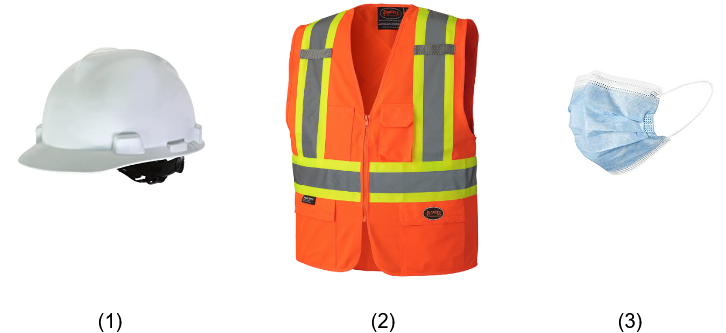
\includegraphics[scale=0.3]{images/ppe.png}}
  	\caption{(1) Mũ bảo hộ, (2) Áo bảo hộ, (3) Khẩu trang}
  	\label{fig:ppe}
\end{figure}

Mục tiêu đầu ra của hệ thống là có thể xác định được vị trí đầu người và thân người và phân loại việc sử dụng các thiết bị bảo hộ cá nhận đối với các vật thể đã được phát hiện. Ứng với mỗi thiết bị, vật thể sẽ được phân loại thành hai trạng thái, một là \emph{Wearing} - \emph{Mặc}, hai là \emph{Not wearing} - \emph{Không mặc}.
\begin{itemize}
	\item Wearing a hardhat
	\item Not wearing a hardhat
	\item Wearing a safety vest
	\item Not wearing a safety vest
	\item Wearing a mask
	\item Not wearing a mask
\end{itemize}
Hình \ref{fig:expected_output} minh họa đầu vào đầu ra mong muốn của hệ thống.
\begin{figure}[ht!]
	\centerline{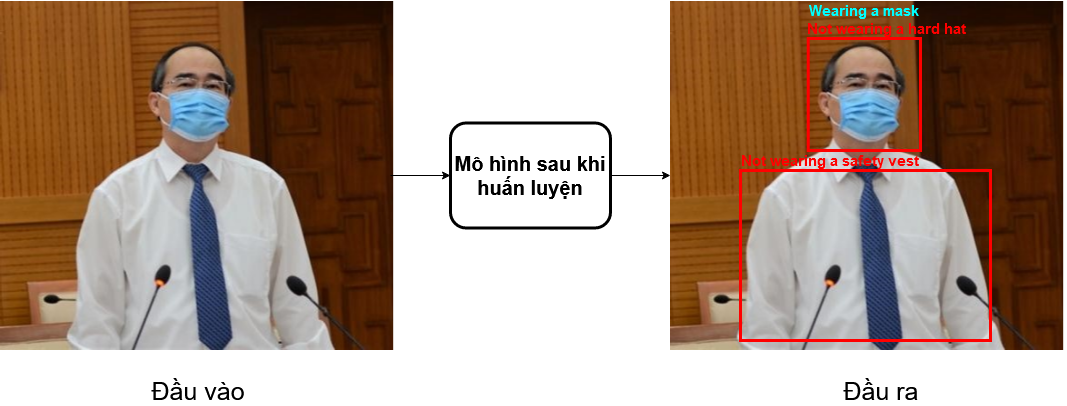
\includegraphics[scale=0.4]{images/expected_output.png}}
  	\caption{Kết quả nhận dạng mong muốn.}
  	\label{fig:expected_output}
\end{figure}

Do vậy tập dữ liệu sẽ được xây dựng với các hình ảnh chứa con người và các nhãn được đánh đúng với mong muốn của đầu ra.
\subsection{Thu thập hình ảnh và dán nhãn}
Tập dữ liệu gồm $11586$ hình trong đó
\begin{itemize}
	\item $3541$ hình được lấy từ tập dữ liệu \emph{Hardhat and Safety Vest Image for Object Detection}\cite{john:2020:hardhat}
	\item $3174$ hình được lấy từ tập dữ liệu \emph{GDUT-HWD}\cite{jixiu:2019:automatic}
	\item $4871$ hình được lấy từ công cụ tìm kiếm hình ảnh \emph{Google image}
\end{itemize}

Các hình được dán nhãn bằng phần mềm \emph{LabelImg}\cite{tzu:2018:labelimg}. Mỗi hình sẽ có tương ứng một tệp tin văn bản với đuôi \emph{.txt}. Bên trong tệp tin này là các nhãn được đánh dấu bằng định dạng của YOLO với các thông tin gồm \emph{object class id} - đây là id tương ứng với thứ tự của một nhãn trong danh sách các nhãn, \emph{x} và \emph{y} là tọa độ tương đối của bounding box được đánh dấu với hình, \emph{w} và \emph{h} là chiều rộng và chiều cao tương đối của bounding box được đánh dấu với hình, hình \ref{fig:yolo_annotation}.
\begin{figure}[ht!]
	\centerline{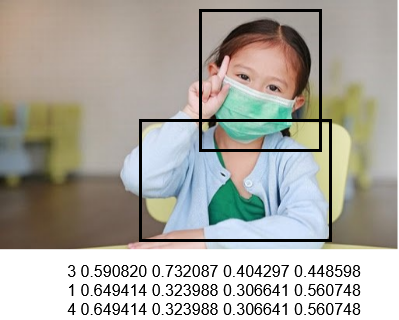
\includegraphics[scale=0.6]{images/yolo_annotation.png}}
  	\caption{Định dạng nhãn của YOLO.}
  	\label{fig:yolo_annotation}
\end{figure}

Tập dữ liệu này có tổng cộng \textbf{195771} vật thể được dán nhãn với thống kê số vật thể của từng class được thể hiện trong hình \ref{fig:object_count}.
\begin{figure}[ht!]
	\centerline{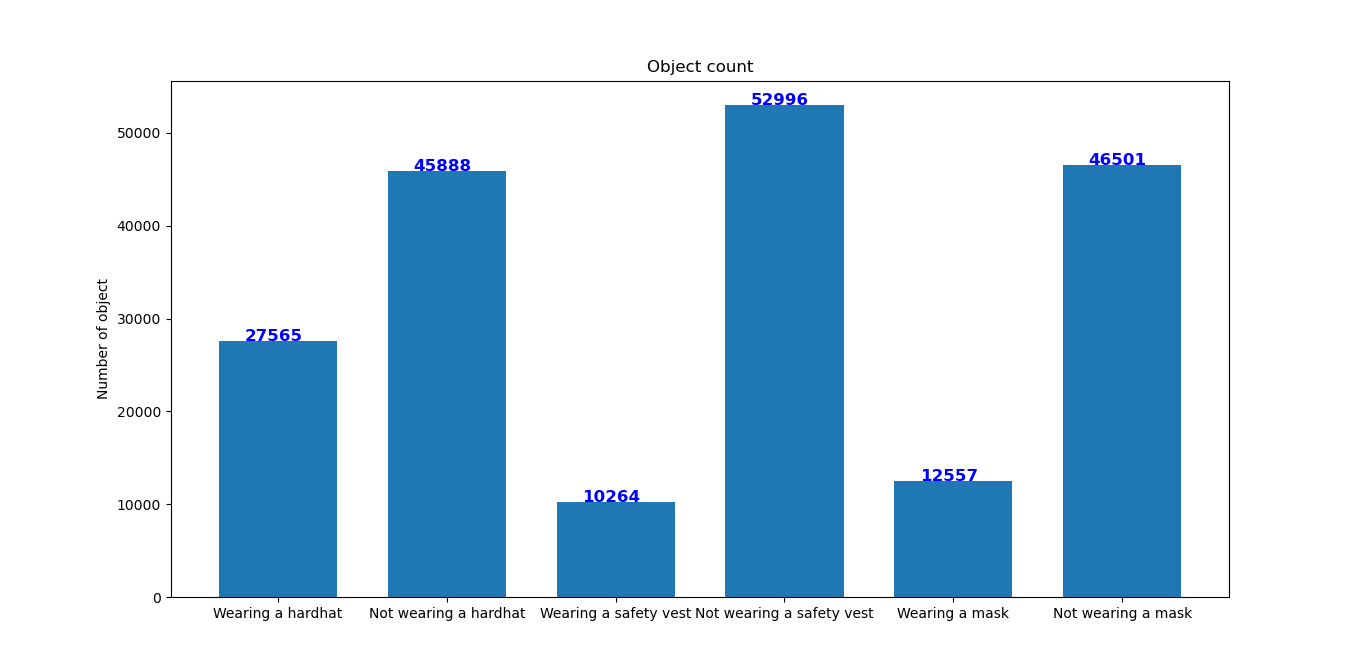
\includegraphics[scale=0.5]{images/object_count.png}}
  	\caption{Thống kê số lượng vật thể ứng với từng class. Wearing a hardhat: $27565$, Not wearing a hardhat: $45888$, Wearing a safety vest: $10264$, Not wearing a safety vest: $52996$, Wearing a mask:$12557$, Not wearing a mask: $46501$.}
  	\label{fig:object_count}
\end{figure}

Việc chênh lệch lớn về số lượng các bounding box giữa các class cụ thể là các class \emph{Not wearing} có số lượng lớn hơn rất nhiều so với các class \emph{Wearing} tương ứng sẽ giúp bộ nhận dạng nhạy hơn với các trường hợp vi phạm trang phục bảo vệ lao động. Tuy có sự chênh lệch lớn nhưng số lượng các bounding box của mỗi class là đủ lớn để mô hình có thể học được các đặc trưng cần thiết để có thể phân loại class tốt cho một bounding box.

\section{Huấn luyên mạng YOLOv3 sử dụng framework Darknet}
Darknet\cite{alexey:2020:darknet} là một framework được xây dựng bởi Joseph Redmon cũng là cha đẻ của YOLO, framework này được viết bằng C/C++ và được dùng để huấn luyện mô hình YOLOv3 với tâp dữ liệu riêng cho từng vấn đề. Kiến trúc của Darknet đã được đề cập ở phần lý thuyết và sẽ không được nhắc lai ở chương này.

Mô hình YOLOv3 trong luận văn này được huấn luyện trên $Google Colab$, về bản chất môi trường trên $Google Colab$ là môi trường máy ảo chạy Linux với các thông số tại thời điểm thực hiện luận văn: 
\begin{itemize}
	\item Hệ điều hành: Ubuntu 18.04.3 LTS
	\item Chip xử lý: Intel 2-core Xeon 2.2GHz
	\item RAM: 13Gb
	\item HDD: 33Gb
	\item GPU: Tesla K80 with 12GB memory
\end{itemize}

Để có thể huấn luyện được mô hình YOLOv3 cho bộ dữ liệu riêng, ta cần thực hiện một số bước.
\begin{enumerate}
	\item Tải framework Darknet từ github repository của \href{https://github.com/AlexeyAB/darknet}{AlexeyAB}.
	
\noindent\fbox{
    \parbox{350pt}{
        https://github.com/AlexeyAB/darknet
    }
}

	Sau đó ta chọn Clone $\rightarrow$ Download ZIP và tiến hành tải thư mục về, sau khi tải xong ta tiến hành giải nén vào một thư mục mà ta tạo sẵn.
	\item Ta chép tệp tin \emph{yolov3.cfg} trong thư mục \emph{cfg} ra thư mục làm việc \emph{darknet} và chỉnh sửa như sau.
	\begin{itemize}
	\item Đầu tiên ta sẽ sửa các giá trị \emph{batch} là số hình trong một mini-batch mà ta muốn dùng để huấn luyện, \emph{subdivision} là thông số để chia nhỏ một mini-batch để đảm bảo mô hình có thể chạy trên các tài nguyên GPU khác nhau, do tập dữ liệu gồm nhiều hình có kích thước khác nhau nên trong quá trình huấn luyện nếu để \emph{subdivision} nhỏ thì rất dễ gặp lỗi \emph{out of memory} do đó sau khi thử nhiều giá trị khác nhau như $16, 32, 64$ thì $64$ cho phép việc training diễn ra tối nhất. Đổi lại thì thời gian training sẽ lâu hơn do không thể đưa nhiều hình vào cùng môt lúc để huấn luyện.	
	\item \emph{width} và \emph{height} là chiều rộng và chiều cao của ảnh đầu vào, các ảnh có kích thước khác nhau sẽ được resize lại kích thước này trước khi được đưa vào để huấn luyện. Việc lựa chọn giá trị \emph{width} và \emph{height} sẽ ảnh hưởng tới việc học của mô hình, nếu như tài nguyên GPU là lớn thì các giá trị của \emph{width} và \emph{height} nên chọn càng lớn càng tốt, tuy nhiên trong bài toán này để đảm bảo hình ảnh sau khi resize không mất quá nhiều thông tin, đồng thời đảm bảo việc huấn luyện có thể thực hiện được trên tài nguyên GPU được cung cấp nên \emph{width} và \emph{height} được chọn là $608$.
	\item Việc lựa chon \emph{max{\_}batches} là tổng số batch mà mô hình sẽ chạy qua, đây còn được gọi là số \emph{iteration}, ta có thể chọn \emph{max{\_}batches} rất lớn và dựa vào \emph{mAP} hoăc \emph{average loss} để dừng giải thuật, nhưng sau khi huấn luyện mô hình một vài lần cho thấy \emph{max{\_}batches} nên xấp xỉ lớn hơn số class nhân $2000$ nhưng không nhỏ hơn số lượng hình trong tập dữ liệu huấn luyện. \emph{steps} sẽ có giá trị lần lượt băng $80\%$ và $90\%$ của \emph{max{\_}batches}.
	\end{itemize}


\noindent\fbox{
    \parbox{350pt}{
        \texttt{\#} [net]\\
		\texttt{\#} Testing\\
		\texttt{\#} batch=1\\
		\texttt{\#} subdivisions=1\\
		\texttt{\#} Training\\
		batch=64\\
		subdivisions=64\\
		width=608\\
		height=608\\
		channels=3\\
		momentum=0.9\\
		decay=0.0005\\
		angle=0\\
		saturation = 1.5\\
		exposure = 1.5\\
		hue=.1\\
\\
		learning{\_}rate=0.001\\
		burn{\_}in=1000\\
		max{\_}batches = 22000\\
		policy=steps\\
		steps=17600,19800\\
		scales=.1,.1\\
    }
}

Sau đó tại các dòng $610, 696$ và $783$ ta sẽ thay số $classes$ bằng sáu, chính là số class của bài toán. Đồng thời ta sẽ sửa số $filters$ của lớp convolution ngay phía trên theo công thức $3 \times (5+C)$ với $C$ là số class, $3$ là số scale mà mô hình sẽ dự đoán, $5$ gồm $4$ tham số tọa độ của bounding box và $1$ tham số dự đoán sự tồn tại của vật thể trong bounding box đó, khi $C=6$ ta có $filters=33$.

\noindent\fbox{
    \parbox{350pt}{
		[convolutional]\\
		size=1\\
		stride=1\\
		pad=1\\
		filters=33\\
		activation=linear\\
\\
		\text{[yolo]}\\
		mask = $0,1,2$\\
		anchors = $10,13,16,30,33,23,30,61,62,45,59,119,116,90,156$ \\ $,198,373,326$\\
		classes=6\\
		num=9\\
		jitter=.3\\
		ignore{\_}thresh = .7\\
		truth{\_}thresh = $1$\\
		random=$1$\\
	}
}

	\item Sửa các thông số ở đầu của tệp \emph{Makefile} như sau. OpenCV và GPU sẽ được sử dụng trong quá trình huấn luyện và dự đoán nên hai giá trị này sẽ được cài đặt là $1$.

\noindent\fbox{
    \parbox{350pt}{
		GPU=1\\
		CUDNN=0\\
		CUDNN{\_}HALF=0\\
		OPENCV=1\\
		AVX=0\\
		OPENMP=0\\
		LIBSO=0\\
		ZED{\_}CAMERA=0 \# ZED SDK 3.0 and above\\
		ZED{\_}CAMERA{\_}v2{\_}8=0 \# ZED SDK 2.X\\
	}
}

	\item Tạo tệp có tên $obj.names$ chứa tên các class.

\noindent\fbox{
    \parbox{350pt}{
		Wearing a hardhat\\
		Not wearing a hardhat\\
		Wearing a safety vest\\
		Not wearing a safety vest\\
		Wearing a mask\\
		Not wearing a mask\
	}
}

	\item Sao chép tập dữ liệu gồm hình ảnh và tệp tin dán nhãn vào đường dẫn \emph{./data/objects}

	\item Tạo hai tệp text, \emph{train.txt} và \emph{val.txt} chứa đường dẫn đến các hình ảnh. \emph{train.txt} sẽ được dùng để huấn luyện còn \emph{val.txt} sẽ được dùng để validate mô hình trong quá trình huấn luyện. Việc chia tập dữ liệu được thực hiện ngẫu nhiên. Có \textbf{900} hình được dùng để validate và \textbf{10686} hình được dùng để huấn luyện. Việc chia này được thực hiện bằng một chương trình Python.

\noindent\fbox{
    \parbox{350pt}{
		import os\\
		import glob\\
		import cv2\\
		import random\\
\\
		basenames = \text{[os.path.basename(x) for x in \\
		\tab glob.glob(".$/$data$/$objects$/$*.jpg")]}\\
		basenamesNotEmpty = []\\

		for name in basenames:\\
		    \tab if "empty" not in name:\\
		    \tab \tab basenamesNotEmpty.append(name)\\

		train = random.sample(basenames, len(basenames))\\
		valid = random.sample(basenamesNotEmpty, 900)\\

		with open(".$/$val.txt","w") as f:\\
    		\tab for name in valid:\\
        		\tab \tab f.write("data$/$objects$/$"+name+"$\backslash$n")\\
        
		with open(".$/$train.txt","w") as f:\\
			\tab for name in train:\\
	        	\tab if name not in valid:\\
		        \tab \tab f.write("data$/$objects$/$"+name+"$\backslash$n")\\
	}
}

	\item Tạo tệp có tên $obj.data$ chứa tên các class.

\noindent\fbox{
    \parbox{350pt}{
		classes = 6\\
		train = train.txt\\
		valid = val.txt\\
		names = obj.names\\
		backup = backup/\\
	}
}

	\item Vào đường dẫn này để tải tệp tin trọng số cho các lớp tích chập được huấn luyện từ mạng Imagenet. Sau đó sao chép tệp tin vừa tải về vào thư mục \emph{darknet}. Tệp tin trọng số \emph{darknet53.conv.74} đã được huấn luyện qua hàng triệu hình nên các trọng số ở các lớp tích chập đã được tối ưu để trích xuất đặc trưng từ hình ảnh. Do vậy ta sẽ tái sử dụng các trọng số ở các lớp tích chập của từ tệp tin trọng số này và chỉ huấn luyện các trọng số ở lớp kết nối đầy đủ cho bài toán của luận văn. Đây là cách làm rất phổ biến vì cho phép kế thừa hiệu năng nhận diện rất tốt của YOLO vào nhiều bài toán nhận diện khác nhau.
	
\noindent\fbox{
    \parbox{350pt}{
	https://pjreddie.com/media/files/darknet53.conv.74
	}
}	
	
	\item Nén thư mục làm việc lại thành một tệp tin \emph{zip}, tạo một thư mục tên \emph{Darknet} trên \emph{Google Drive} và upload tệp tin đã nén vào thư mục này. Đồng thời tạo một thư mục con có tên \emph{backup} trong \emph{Darknet}.
	
	\item Trong \emph{Google Colab}, chọn \emph{Runtime} $\rightarrow$ \emph{Change runtime type} $\rightarrow$ \emph{Hardware accelerator} $\rightarrow$ \emph{GPU}, chạy đoạn code sau để \emph{build Darknet}.

\noindent\fbox{
    \parbox{350pt}{
	from google.colab import drive\\
	drive.mount('/content/drive')\\
	{\%}cd /content\\
	!unzip /content/drive/'My Drive'/Darknet/darknet.zip\\
	{\%}cd /content/darknet\\
	!sudo apt-get install dos2unix\\
	!make\\
	!chmod +x ./darknet\\
	!rm /content/darknet/backup -r\\
	!ln -s /content/drive/'My Drive'/Darknet/backup /content/darknet\\
	{\%}cd /content/darknet\\
	!find . -type f -name "*.txt" -print0 | xargs -0 dos2unix\\
	}
}

	\item Đối với lần đầu tiên ta sẽ chạy dòng lệnh sau.
	
\noindent\fbox{
    \parbox{350pt}{
	!./darknet detector train obj.data yolov3.cfg darknet53.conv.74
	}
}	

	Đối với các lần huấn luyện sau ta chỉ cần dùng tệp tin \emph{yolov3{\_}last.weights} để huấn luyện tiếp mà không cần huấn luyện lại từ đầu.
	
\noindent\fbox{
    \parbox{350pt}{
	!./darknet detector train obj.data yolov3.cfg ./backup/yolov3{\_}last.weights
	}
}

	\item \emph{Darknet} sẽ tự động lưu các tệp tin trọng số mỗi $1000$ \emph{iteration} ví dụ: \emph{yolov3{\_}1000.weights}, \emph{yolov3{\_}2000.weights}. Ta có thể dừng việc huấn luyện để kiểm tra các tham số hiệu năng của mô hình như \emph{precision} và \emph{recall}. Việc kiểm tra này được thực hiện trên tập dữ liệu validate trong tệp \emph{val.txt}. Để thực hiện việc kiểm tra này ta sẽ chạy dòng lệnh sau.
	
\noindent\fbox{
    \parbox{350pt}{
	!./darknet detector map obj.data yolov3.cfg ./backup/yolov3{\_}1000.weights
	}
}

	Ta có thể thay \emph{yolov3{\_}1000.weights} bằng tệp tin trọng số mà ta muốn kiểm tra.
\end{enumerate}

\section{Sử dụng mô hình YOLOv3 để nhận diện trên camera hoặc video}

Sau khi việc huấn luyện đã hoàn thành, ta sẽ dùng tệp tin trọng số để tiến hành nhận diện trên video hoặc camera. Để làm được điều này ta sẽ viết một chương trình Python có sơ đồ khối như hình \ref{fig:flow_chart}.
\begin{figure}[ht!]
	\centerline{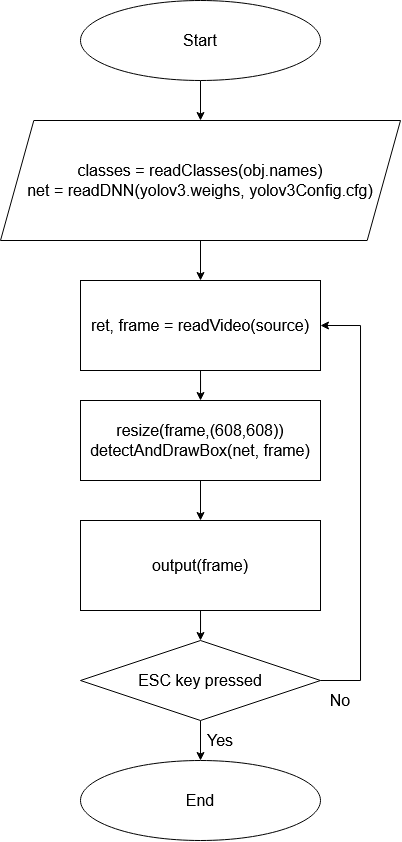
\includegraphics[scale=0.6]{images/flow_chart.png}}
  	\caption{Sơ đồ khối chương trình Python để nhận dạng trên video hoặc webcam.}
  	\label{fig:flow_chart}
\end{figure}

\begin{enumerate}
	\item Chương trình sẽ lấy tên các class được đinh nghĩa sẵn trong tệp tin \emph{obj.names}, đồng thời sẽ đọc các giá trị trọng số của mô hình trong tệp tin \emph{yolov3.weights} dựa trên các thông số về kiến trúc đã cài đặt trong tệp tin \emph{yolov3Config.cfg}. Hàm để đọc mô hình DNN trong OpenCV là \emph{cv2.dnn.readNet(weightsFile, configFile)} với \emph{weightsFile} là tệp tin trọng số và \emph{configFile} là tệp tin kiến trúc của mạng.
	
	\item Sau đó ta sẽ dùng hàm đọc video của OpenCV để đọc dữ liệu từ webcam. Đầu tiên ta sẽ khởi tạo một đối tượng đại diện cho webcam \emph{cap = VideoCapture(0)}. Sau đó ta sẽ đọc từng frame từ đối tượng vừa được khởi tạo \emph{ret, image = cap.read()} với \emph{image} là biến chứa một frame, \emph{ret} sẽ có giá trị \emph{True} nếu có frame được đọc từ đầu vào và \emph{False} nếu không có frame được đọc từ đầu vào.
	
	\item Để tiến hành nhận dạng trên hình, ta sẽ dùng các câu lệnh sau.

\noindent\fbox{
    \parbox{350pt}{
    blob = cv2.dnn.blobFromImage(image, scale, (604, 604), (0, 0, 0), \\ \tab True, crop=False)\\
	net.setInput(blob)\\
    outs = net.forward(get{\_}output{\_}layers(net))\\
	}
}

	Dòng lênh đầu tiên sẽ resize hình về kích thước $(604, 604)$, hiện nay các camera quan sát thường có độ phân giải 2MP với kích thước khung hình $1920 \times 1080$ nên việc resize về $604 \times 604$ sẽ không làm mất đi các đặc trưng quan trọng và cho phép giảm thiểu số lượng tính toán để việc dự đoán trên hình nhanh hơn và tốn ít tài nguyên phần cứng hơn. Sau đó từng pixel trong hình sẽ được trừ cho $(0, 0, 0)$ và chia cho \emph{scale}. \emph{swapRB=True} sẽ hoán đổi vị trí hai kênh đỏ và xanh dương trong tensor của hình. \emph{crop=False} sẽ không crop hình sau khi resize. Giả sử kênh màu đỏ của hình sau khi được resize có giá trị là $R$, \emph{scale}$=\sigma$, giá trị để trừ là ${\mu}_{red}$, giá trị của kênh màu đỏ sau khi đi qua hàm \emph{blob} sẽ là
\begin{equation}
	\frac{R-{\mu}_{red}}{\sigma}
\end{equation} 
	Kết quả của hàm \emph{blob} sẽ được đưa vào đối tượng \emph{net} và đầu ra sẽ là kết quả của quá trình feed forward.
	
	\item Tuy nhiên tại đầu ra \emph{outs} sẽ có rất nhiều bounding box bị trùng lặp do với cũng một vật thể và class. Do đó kết quả đầu ra cần phải đi qua giải thuật non-maximum suppression để có thể lấy một bounding box riêng biệt và duy nhất cho một vật thể.
	
	Về cơ bản giải thuật non-maximum suppression hoạt động như sau.
	\begin{enumerate}
		\item Bắt đầu giải thuật có sẽ có hai mảng một chiều A và B với mảng A chứa các bounding box cần xử lý, mảng B rỗng.
		\item Lấy bounding box có giá trị \emph{confidence} lớn nhất trong A và đưa vào B và loại bounding box này ra khỏi A.
		\item Với mọi bounding box còn lại trong A, tìm IOU với bounding box vừa đưa vào B. Nếu IOU lớn hơn ngưỡng \emph{nmsThreshold} thì loại bounding đang xét ra khỏi A.
		\item Lặp lại bước (b) và (c) cho đến khi không còn bounding box nào trong A.
	\end{enumerate}

\noindent\fbox{
    \parbox{350pt}{
	indices = cv2.dnn.NMSBoxes(boxes, confidences, confThreshold, nmsThreshold)
	}
}

	\item Cuối cùng, ta sẽ vẽ các bounding box vào frame và xuất ra màn hình.

\noindent\fbox{
    \parbox{350pt}{
    for i in indices:\\
    \tab i = i[0]\\
    \tab box = boxes[i]\\
    \tab x = box[0]\\
    \tab y = box[1]\\
    \tab w = box[2]\\
    \tab h = box[3]\\
    \tab image = draw{\_}prediction(image, class{\_}ids[i], confidences[i], round(x), round(y), round(x + w), round(y + h))\\
\\
    cv2.imshow("test", image)
	}
}

Chương trình Python để sau cùng để nhận diện trên webcam.

\noindent\fbox{
    \parbox{350pt}{
from PIL import Image
\\import time
\\import cv2
\\import argparse
\\import numpy as np
\\
\\def get{\_}output{\_}layers(net):
\\\tab layer{\_}names = net.getLayerNames()
\\
\\\tab output{\_}layers = [layer{\_}names[i[0] - 1] for i in net.getUnconnectedOutLayers()]
\\
\\\tab return output{\_}layers
\\
\\
\\def draw{\_}prediction(img, class{\_}id, confidence, x, y, x{\_}plus{\_}w, y{\_}plus{\_}h):
\\\tab label = str(classes[class{\_}id])
\\
\\\tab if class{\_}id == 5 or class{\_}id == 3 or class{\_}id == 1:
\\\tab \tab color = [0,0,255]
\\\tab else:
\\\tab \tab color = COLORS[class{\_}id]
\\\tab 
\\\tab cv2.rectangle(img, (x, y), (x{\_}plus{\_}w, y{\_}plus{\_}h), color, 2)
\\
\\\tab if class{\_}id == 5 or class{\_}id == 4:
\\\tab \tab cv2.putText(img, label, (x - 10, y - 35), cv2.FONT{\_}HERSHEY{\_}SIMPLEX, 1, color, 1)
\\\tab else:
\\\tab \tab cv2.putText(img, label, (x - 10, y - 10), cv2.FONT{\_}HERSHEY{\_}SIMPLEX, 1, color, 1)
\\
\\\tab return img
	}
}

\noindent\fbox{
    \parbox{355pt}{
def eudistance(v1, v2):
\\\tab dist = [(a - b)**2 for a, b in zip(v1, v2)]
\\\tab dist = math.sqrt(sum(dist))
\\\tab return dist
\\
\\{\#} Create a VideoCapture object
\\cap = cv2.VideoCapture(0)
\\
\\{\#} Check if camera opened successfully
\\if (cap.isOpened() == False): 
\\\tab print("Unable to read camera feed")
\\
\\{\#} Default resolutions of the frame are obtained.The default resolutions are system dependent.
\\{\#} We convert the resolutions from float to integer.
\\frame{\_}width = int(cap.get(3))
\\frame{\_}height = int(cap.get(4))
\\
\\classes = []
\\with open("obj.names", 'r') as f:
\\\tab classes = [line.strip() for line in f.readlines()]
\\
\\COLORS=[[0,128,0],[255,0,0],[255,165,0],[0,0,255],[255,255,0],[255,69,0]]
\\
\\
\\net = cv2.dnn.readNet("yolov3-tiny{\_}12000.weights", "yolov3-tiny.cfg")
\\
\\conf{\_}threshold = 0.2
\\nms{\_}threshold = 0.4
\\
\\
\\Width = frame{\_}width
\\Height = frame{\_}height
\\scale = 0.00392
	}
}

\noindent\fbox{
    \parbox{350pt}{
start = time.time()
\\count = 0
\\while(True):
\\\tab ret, image = cap.read()
\\
\\\tab if ret == True: 
\\\tab \tab if count % 3 == 0:
\\\tab \tab \tab blob = cv2.dnn.blobFromImage(image, scale, (604, 604), (0, 0, 0), True, crop=False)
\\
\\\tab \tab \tab net.setInput(blob)
\\
\\\tab \tab \tab outs = net.forward(get{\_}output{\_}layers(net))
\\\tab \tab \tab 
\\\tab \tab \tab class{\_}ids = []
\\\tab \tab \tab confidences = []
\\\tab \tab \tab boxes = []
\\\tab \tab \tab class{\_}ids{\_}mask = []
\\\tab \tab \tab confidences{\_}mask = []
\\\tab \tab \tab boxes{\_}mask = []
\\\tab \tab \tab class{\_}ids{\_}hat = []
\\\tab \tab \tab confidences{\_}hat = []
\\\tab \tab \tab boxes{\_}hat = []
\\
\\\tab \tab \tab for out in outs:
\\\tab \tab \tab \tab for detection in out:
\\\tab \tab \tab \tab \tab scores = detection[5:]
\\\tab \tab \tab \tab \tab class{\_}id = np.argmax(scores)
\\\tab \tab \tab \tab \tab confidence = scores[class{\_}id]
\\\tab \tab \tab \tab \tab if class{\_}id == 0 or class{\_}id == 1 or class{\_}id == 4 or class{\_}id == 5:
\\\tab \tab \tab \tab \tab \tab mask{\_}id = 0
\\\tab \tab \tab \tab \tab \tab hat{\_}id = 0
\\\tab \tab \tab \tab \tab \tab 
\\\tab \tab \tab \tab \tab \tab if float(scores[0]) > float(scores[1]):
\\\tab \tab \tab \tab \tab \tab \tab hat{\_}id = 0
\\\tab \tab \tab \tab \tab \tab else:
\\\tab \tab \tab \tab \tab \tab \tab hat{\_}id = 1
	}
}

\noindent\fbox{
    \parbox{350pt}{
\tab \tab \tab \tab \tab \tab if float(scores[4]) > float(scores[5]):
\\\tab \tab \tab \tab \tab \tab \tab mask{\_}id = 4
\\\tab \tab \tab \tab \tab \tab else:
\\\tab \tab \tab \tab \tab \tab \tab mask{\_}id = 5
\\\tab \tab \tab \tab \tab \tab 
\\\tab \tab \tab \tab \tab \tab if confidence > 0.25:
\\\tab \tab \tab \tab \tab \tab \tab center{\_}x = int(detection[0] * Width)
\\\tab \tab \tab \tab \tab \tab \tab center{\_}y = int(detection[1] * Height)
\\\tab \tab \tab \tab \tab \tab \tab w = int(detection[2] * Width)
\\\tab \tab \tab \tab \tab \tab \tab h = int(detection[3] * Height)
\\\tab \tab \tab \tab \tab \tab \tab x = center{\_}x - w / 2
\\\tab \tab \tab \tab \tab \tab \tab y = center{\_}y - h / 2
\\\tab \tab \tab \tab \tab \tab \tab 
\\\tab \tab \tab \tab \tab \tab \tab class{\_}ids{\_}mask.append(mask{\_}id)
\\\tab \tab \tab \tab \tab \tab \tab confidences{\_}mask.append(float(scores[hat{\_}id]))
\\\tab \tab \tab \tab \tab \tab \tab boxes{\_}mask.append([x, y, w, h])
\\\tab \tab \tab \tab \tab \tab \tab 
\\\tab \tab \tab \tab \tab \tab \tab class{\_}ids{\_}hat.append(hat{\_}id)
\\\tab \tab \tab \tab \tab \tab \tab confidences{\_}hat.append(float(scores[hat{\_}id]))
\\\tab \tab \tab \tab \tab \tab \tab boxes{\_}hat.append([x, y, w, h])
\\
\\\tab \tab \tab \tab \tab else:
\\\tab \tab \tab \tab \tab \tab if confidence > 0.25:
\\\tab \tab \tab \tab \tab \tab \tab center{\_}x = int(detection[0] * Width)
\\\tab \tab \tab \tab \tab \tab \tab center{\_}y = int(detection[1] * Height)
\\\tab \tab \tab \tab \tab \tab \tab w = int(detection[2] * Width)
\\\tab \tab \tab \tab \tab \tab \tab h = int(detection[3] * Height)
\\\tab \tab \tab \tab \tab \tab \tab x = center{\_}x - w / 2
\\\tab \tab \tab \tab \tab \tab \tab y = center{\_}y - h / 2
\\\tab \tab \tab \tab \tab \tab \tab class{\_}ids.append(class{\_}id)
\\\tab \tab \tab \tab \tab \tab \tab confidences.append(float(scores[class{\_}id]))
\\\tab \tab \tab \tab \tab \tab \tab boxes.append([x, y, w, h])
\\
\\\tab \tab \tab indices = cv2.dnn.NMSBoxes(boxes, confidences, conf{\_}threshold, nms{\_}threshold)
\\\tab \tab \tab indices{\_}mask = cv2.dnn.NMSBoxes(boxes{\_}mask, confidences{\_}mask, conf{\_}threshold, nms{\_}threshold)
	}
}

\noindent\fbox{
    \parbox{350pt}{
\tab \tab \tab indices{\_}hat = cv2.dnn.NMSBoxes(boxes{\_}hat, confidences{\_}hat, conf{\_}threshold, nms{\_}threshold)
\\\tab \tab 
\\\tab \tab for i in indices:
\\\tab \tab \tab i = i[0]
\\\tab \tab \tab box = boxes[i]
\\\tab \tab \tab x = box[0]
\\\tab \tab \tab y = box[1]
\\\tab \tab \tab w = box[2]
\\\tab \tab \tab h = box[3]
\\\tab \tab \tab image = draw{\_}prediction(image, class{\_}ids[i], confidences[i], round(x), round(y), round(x + w), round(y + h))
\\
\\\tab \tab for i in indices{\_}mask:
\\\tab \tab \tab i = i[0]
\\\tab \tab \tab if class{\_}ids{\_}mask[i] == 5:
\\\tab \tab \tab \tab noMask = True
\\\tab \tab \tab else:
\\\tab \tab \tab \tab noMask = False
\\\tab \tab \tab box = boxes{\_}mask[i]
\\\tab \tab \tab x = box[0]
\\\tab \tab \tab y = box[1]
\\\tab \tab \tab w = box[2]
\\\tab \tab \tab h = box[3]
\\\tab \tab \tab image = draw{\_}prediction(image, class{\_}ids{\_}mask[i], confidences{\_}mask[i], round(x), round(y), round(x + w), round(y + h))
	}
}

\noindent\fbox{
    \parbox{350pt}{
\tab \tab for i in indices{\_}hat:
\\\tab \tab \tab i = i[0]
\\\tab \tab \tab if class{\_}ids{\_}hat[i] == 1:
\\\tab \tab \tab \tab noHat = True
\\\tab \tab \tab else:
\\\tab \tab \tab \tab noHat = False
\\\tab \tab \tab box = boxes{\_}hat[i]
\\\tab \tab \tab x = box[0]
\\\tab \tab \tab y = box[1]
\\\tab \tab \tab w = box[2]
\\\tab \tab \tab h = box[3]
\\\tab \tab \tab image = draw{\_}prediction(image, class{\_}ids{\_}hat[i], confidences{\_}hat[i], round(x), round(y), round(x + w), round(y + h))
\\\tab \tab 
\\\tab \tab cv2.putText(image, "FPS: "+ str(round(count/(time.time()-start))), (30, 30), cv2.FONT{\_}HERSHEY{\_}SIMPLEX, 1, [0,255,0], 1)
\\\tab \tab {\#} Show webcam
\\\tab \tab cv2.imshow("test", image)
\\
\\\tab k = cv2.waitKey(1)\tab  
\\\tab if k%256 == 27:
\\\tab \tab {\#} ESC pressed
\\\tab \tab print("Escape hit, closing...")
\\\tab \tab break
\\\tab count+=1
\\
\\cap.release()
\\cv2.destroyAllWindows()
\\
\\end = time.time()
\\print("YOLO Execution time: " + str(end-start))
	}
}

\end{enumerate}

Chương \emph{Phương pháp tiếp cận} đã trình bày các bước để ứng dụng mô hình mạng neuron tích chập YOLOv3 để giải quyết bài toán nhận diện trang phục bảo hộ lao động. Bắt đầu từ việc xây dựng tập dữ liệu theo format của YOLO, sau đó huấn luyện sử dụng framework darknet, sau cùng là sử dụng mô hình đã huấn luyện được vào chương trình Python. Tuy nhiên, đối với các bài toán ứng dụng trí tuệ nhân tạo, việc đánh giá các thông số hiệu năng của mô hình là vô cùng quan trọng, do vậy chương sau sẽ được dành để đánh giá các thông số hiệu năng của mô hình đã được huấn luyện.